\section{Cartes}

\subsection{Emetteur}
\normalsize
Vous trouverez page suivante le sch�ma de la carte �mettrice. Celle qui mesure la temp�rature. Pour un soucis de consommation, plusieurs r�gulateurs avec "Enable" ont �t� utilis�s pour pouvoir couper l'alimentation de tout ce qui est inutile � certain moment.

Puis les pages suivantes sont directement tir�e du fichier PostScript export� par Pcb. Il s'agit des typons de la carte �mettrice. 

\subsection{R�cepteur}
Ensuite vous trouverez le sch�ma de la carte r�cepteur. Bien remarquer le condensateur de 470~nF. C'est par lui qu'est fix� le potentiel 3,3~V pour fixer la vitesse de transmission sur la liaison USB. 

Puis les typons de la carte r�cepteur export�s par Pcb. 3 feuilles parmis 12 (masque, trou de per�age, \dots)

\begin{landscape}
\begin{figure}[h]
    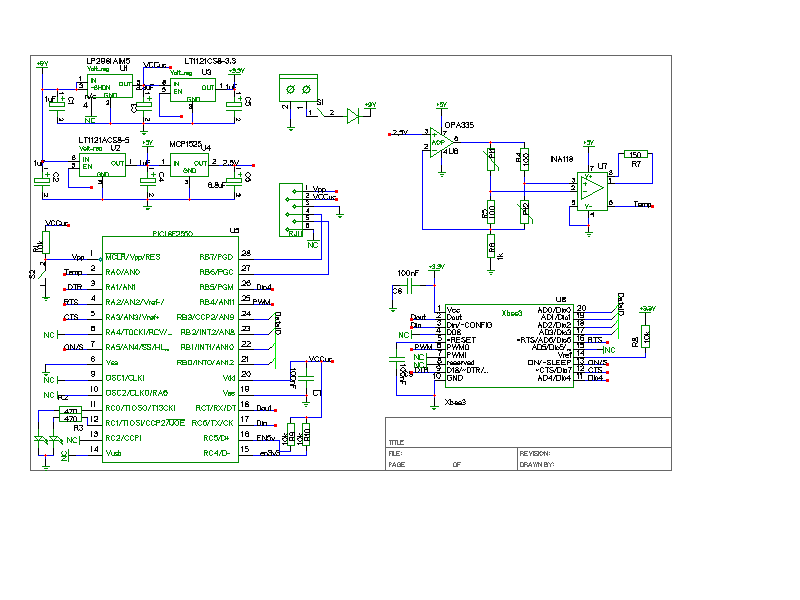
\includegraphics[width=25cm]{./img/Emet}
    \caption{Schema \' Emetteur}
\end{figure}
\end{landscape}

\includepdf[pages={2,3,11},pagecommand={\thispagestyle{plain}}]{Emetteur} 



\begin{landscape}
\begin{figure}[]
    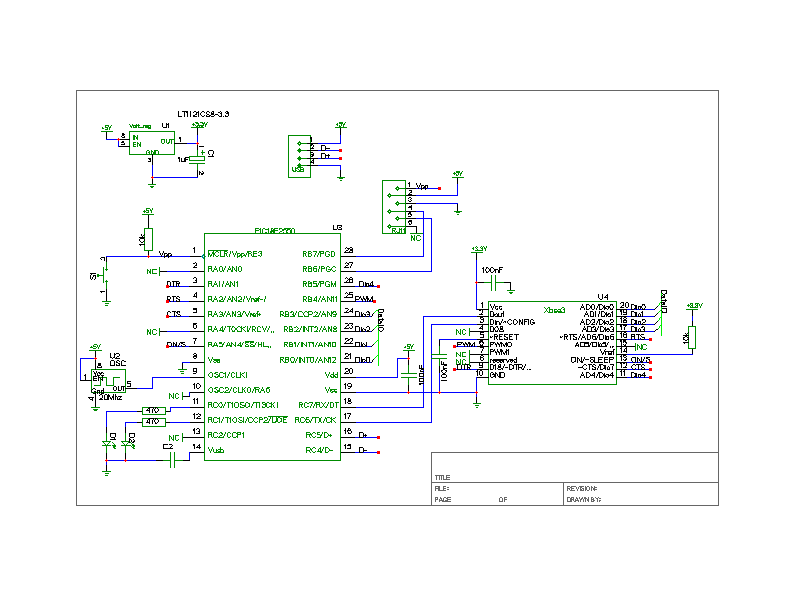
\includegraphics[width=25cm]{./img/Recep}
    \caption{Schema \' Emetteur}
\end{figure}
\end{landscape}
\includepdf[pages={2,3,11},pagecommand={\thispagestyle{plain}}]{Recepteur} 
